\documentclass[../summary.tex]{subfiles}

\begin{document}
	
	\section{Biodiversity}
	
	\subsection{Study guide}
	
	Module 2 (Biodiversity) sketches basic insights biodiversity, different types of diversity, in an historical perspective and with options for the future. Make sure to understand:
	\begin{itemize}
		\setlength{\itemsep}{0pt}
		\item The different types of diversity
		\item Historical evolution of biodiversity
		\item The importance of biodiversity
		\item How biodiversity can be measured and what the challenges in this are
		\item The important treats for biodiversity
		\item Different options to restore biodiversity
		\item Being able to interpret data with regard to biodiversity
	\end{itemize} 
	\ \\
	Don’t learn the specific examples by heart, do not learn specific vocabulary by heart (such as Cambrian or Cretaceous).
	\\
	
	\subsection{Types of diversity}
	First, we need to define what \textbf{biodiversity} actually means. It is the variability among living organisms from all sources, including, inter alia, terrestrial, marine and other aquatic ecosystems and the ecological complexes of which they are parts. This includes the diversity within species, between species and of ecosystems
	\\
	\\
	The first type of biodiversity is \textbf{genetic diversity} or diversity within species. It is the amount of naturally occurring genetic variation among individuals of the same species. 
	\\
	\\
	Another type of diversity is \textbf{species diversity}. This type is often defined as the number of species at a certain location. Figure \ref{fig:diversity_species} gives an indication of this diversity.
	\\
	\\
	Thirdly, there also is \textbf{diversity in ecosystems}. There are a lot of different ecosystems around the globe: from the boreal forest at high latitudes to tropical forests around the equator, but also aquatic ecosystems like lake systems, coral reefs and mangroves count towards ecosystem diversity.
	\\
	\begin{figure}[H]
		\centering
		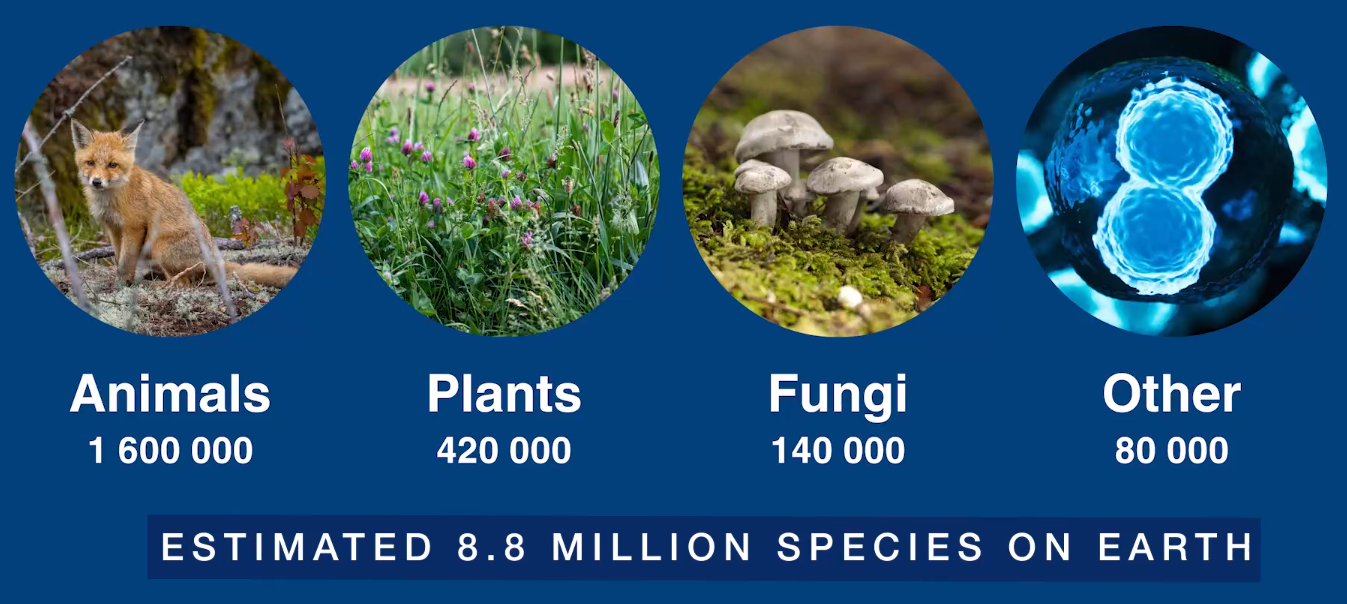
\includegraphics[width=0.75\linewidth]{images/2-diversity_species.png}
		\caption{Diversity in species}
		\label{fig:diversity_species}
	\end{figure}
	
	\subsection{Historical evolution of biodiversity}

	First, it is useful to mention that the plant Earth is about 4.5 billion years old and the first bacterial life emerged about 3.7 billion years ago. We can see the \textbf{increase} of both \textbf{terrestrial species} and \textbf{marine species} through time. The first vertebrates (notably fish) appeared 500 million years ago, the land plants 470 million years ago and the mammals 200 million years ago. Figure \ref{fig:historical-evolution-of-biodiversity} shows this increase over time.
	
	\begin{figure}[H]
		\centering
		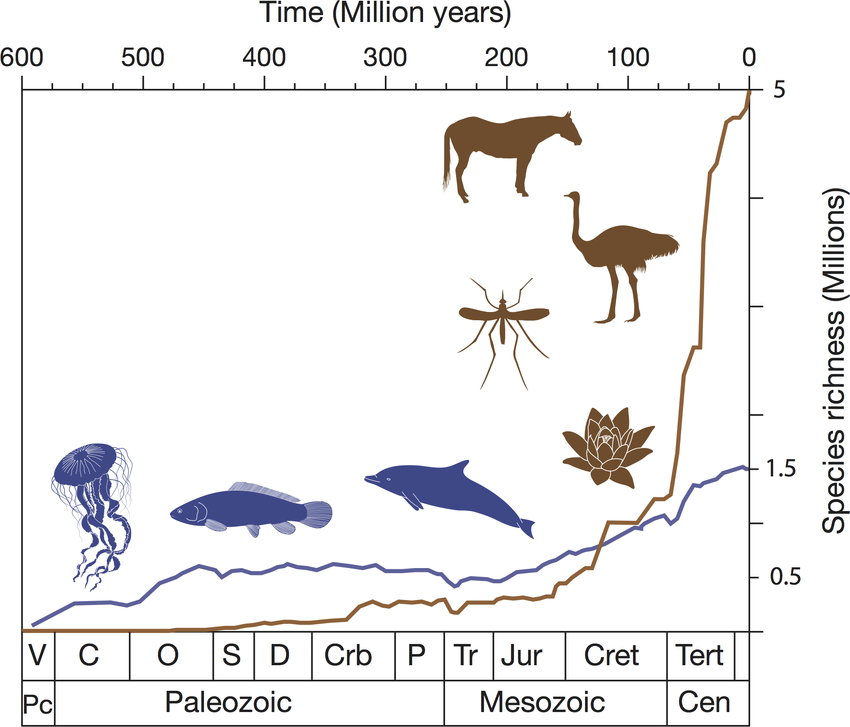
\includegraphics[width=0.45\linewidth]{../images/2-historical-evolution-of-biodiversity}
		\caption{Increase of diversity and number of species over time}
		\label{fig:historical-evolution-of-biodiversity}
	\end{figure}
	\ \\
	The process behind the increasing species richness through time is \textbf{speciation}. This is the evolutionary process by which different populations of the same species evolve to become distinct species. Today's species richness is only a fraction (between 2\% and 5\%) of the number of species ever present on Earth. Many species became extinct, either for no really identifiable reason (these are the so-called \textbf{background extinctions}) or as a result of a large-scale catastrophes (these are the \textbf{mass extinctions}).
	\\
	\\
	Population declines of living species are hidden from global extinction numbers, but are shown in, for example, the \textbf{Living Planet Index}. This measure shows the evolution of the average population size of 21,000 animal populations across the globe. The living planet index shows a dramatic decline of 69\% since the start in 1970.  A problem with this index is that it gives no information about the fate of individual species, and that it is affected by a minority of populations with a strong negative trend.
	
	\begin{figure}[H]
		\centering
		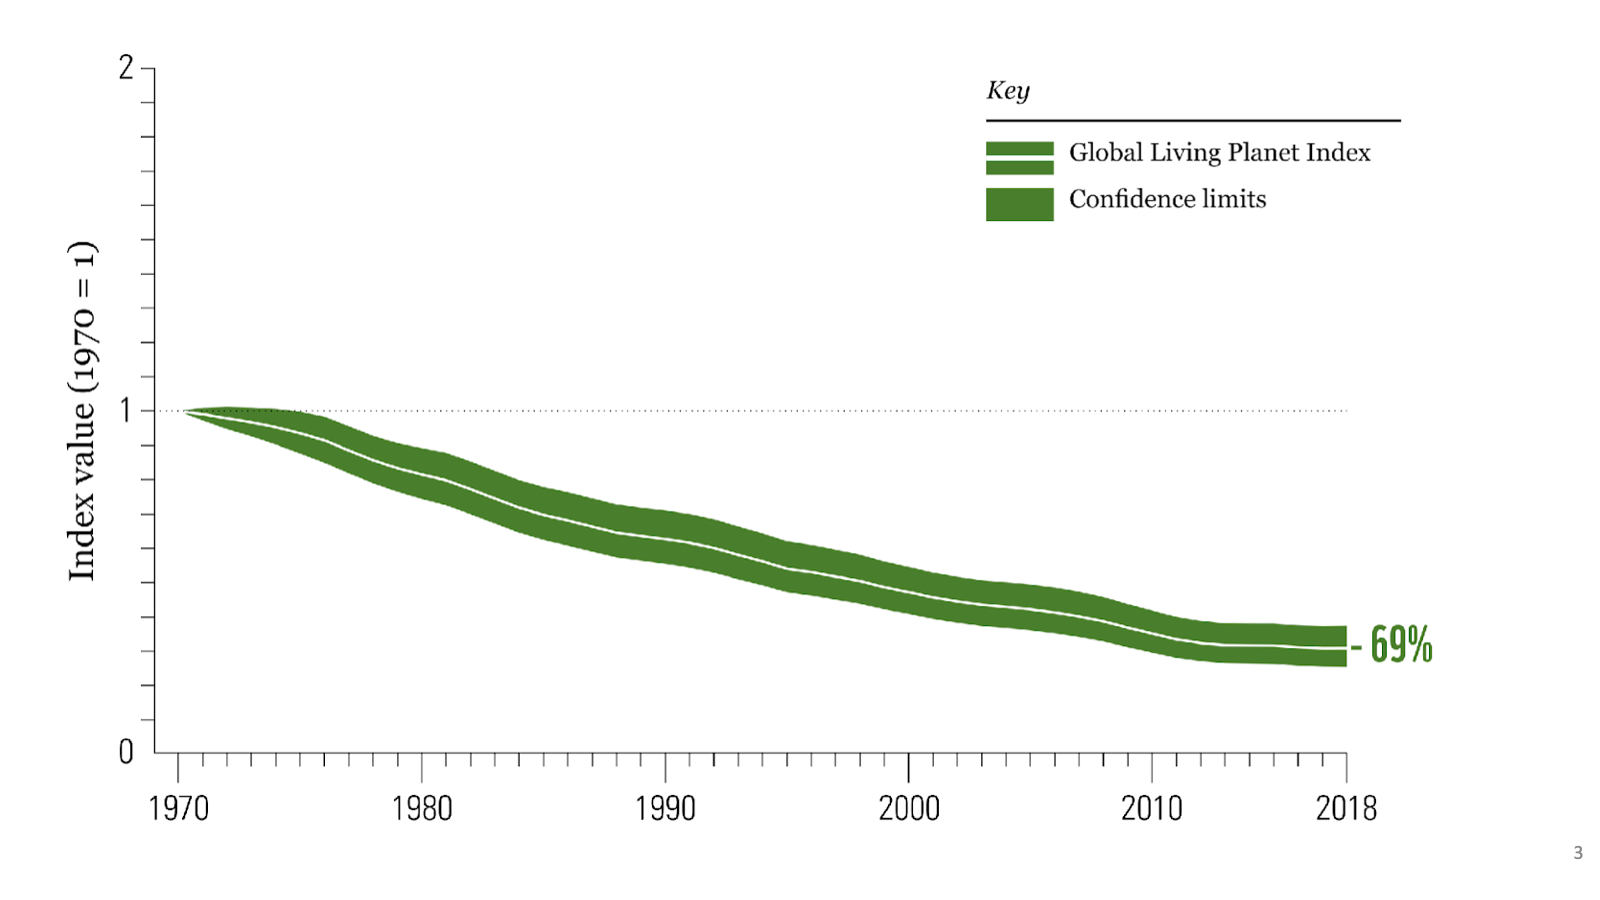
\includegraphics[width=0.7\linewidth]{../images/2-living-planet-index}
		\caption{Living Planet Index}
		\label{fig:living-planet-index}
	\end{figure}
	
	
	\subsection{The importance of biodiversity}
	The human society depends on nature for its ecosystem services. \textbf{Ecosystem Services are the goods and services humans get from ecosystems}. This continuous and vital flow of ecosystem services from ecosystems to humans can be visualized by the ecosystem services cascade.
	\\
	\\
	In the Ecosystem Services cascade of Figure \ref{fig:ecosystems_services_cascade}, we see the integrated social-ecological system with to the left the ecosystem and to the right the human society. The ecosystem has its composition, structure and function, which all are determined by its biodiversity. The human society receives a flow of ecosystem services from the ecosystem, which contribute to the prosperity and well-being of its members. 
	\\
	\\
	Ecosystem Services can be divided in three main categories: provisioning, regulating and cultural services. The \textbf{provisioning services} consist of the material flows, like agricultural crops for food, wood for construction, biomass for energy or drinking water. \textbf{Regulating services} are those that provide environmental protection like erosion control, air cooling and filtering by vegetation or climate mitigation through carbon uptake and storage in forests, peatlands and soils. \textbf{Cultural services} include the diverse spiritual, recreational and scientific experiences ecosystems provide to humans. All these services directly depend on biodiversity.
	
	\begin{figure}[htbp]
		\centering
		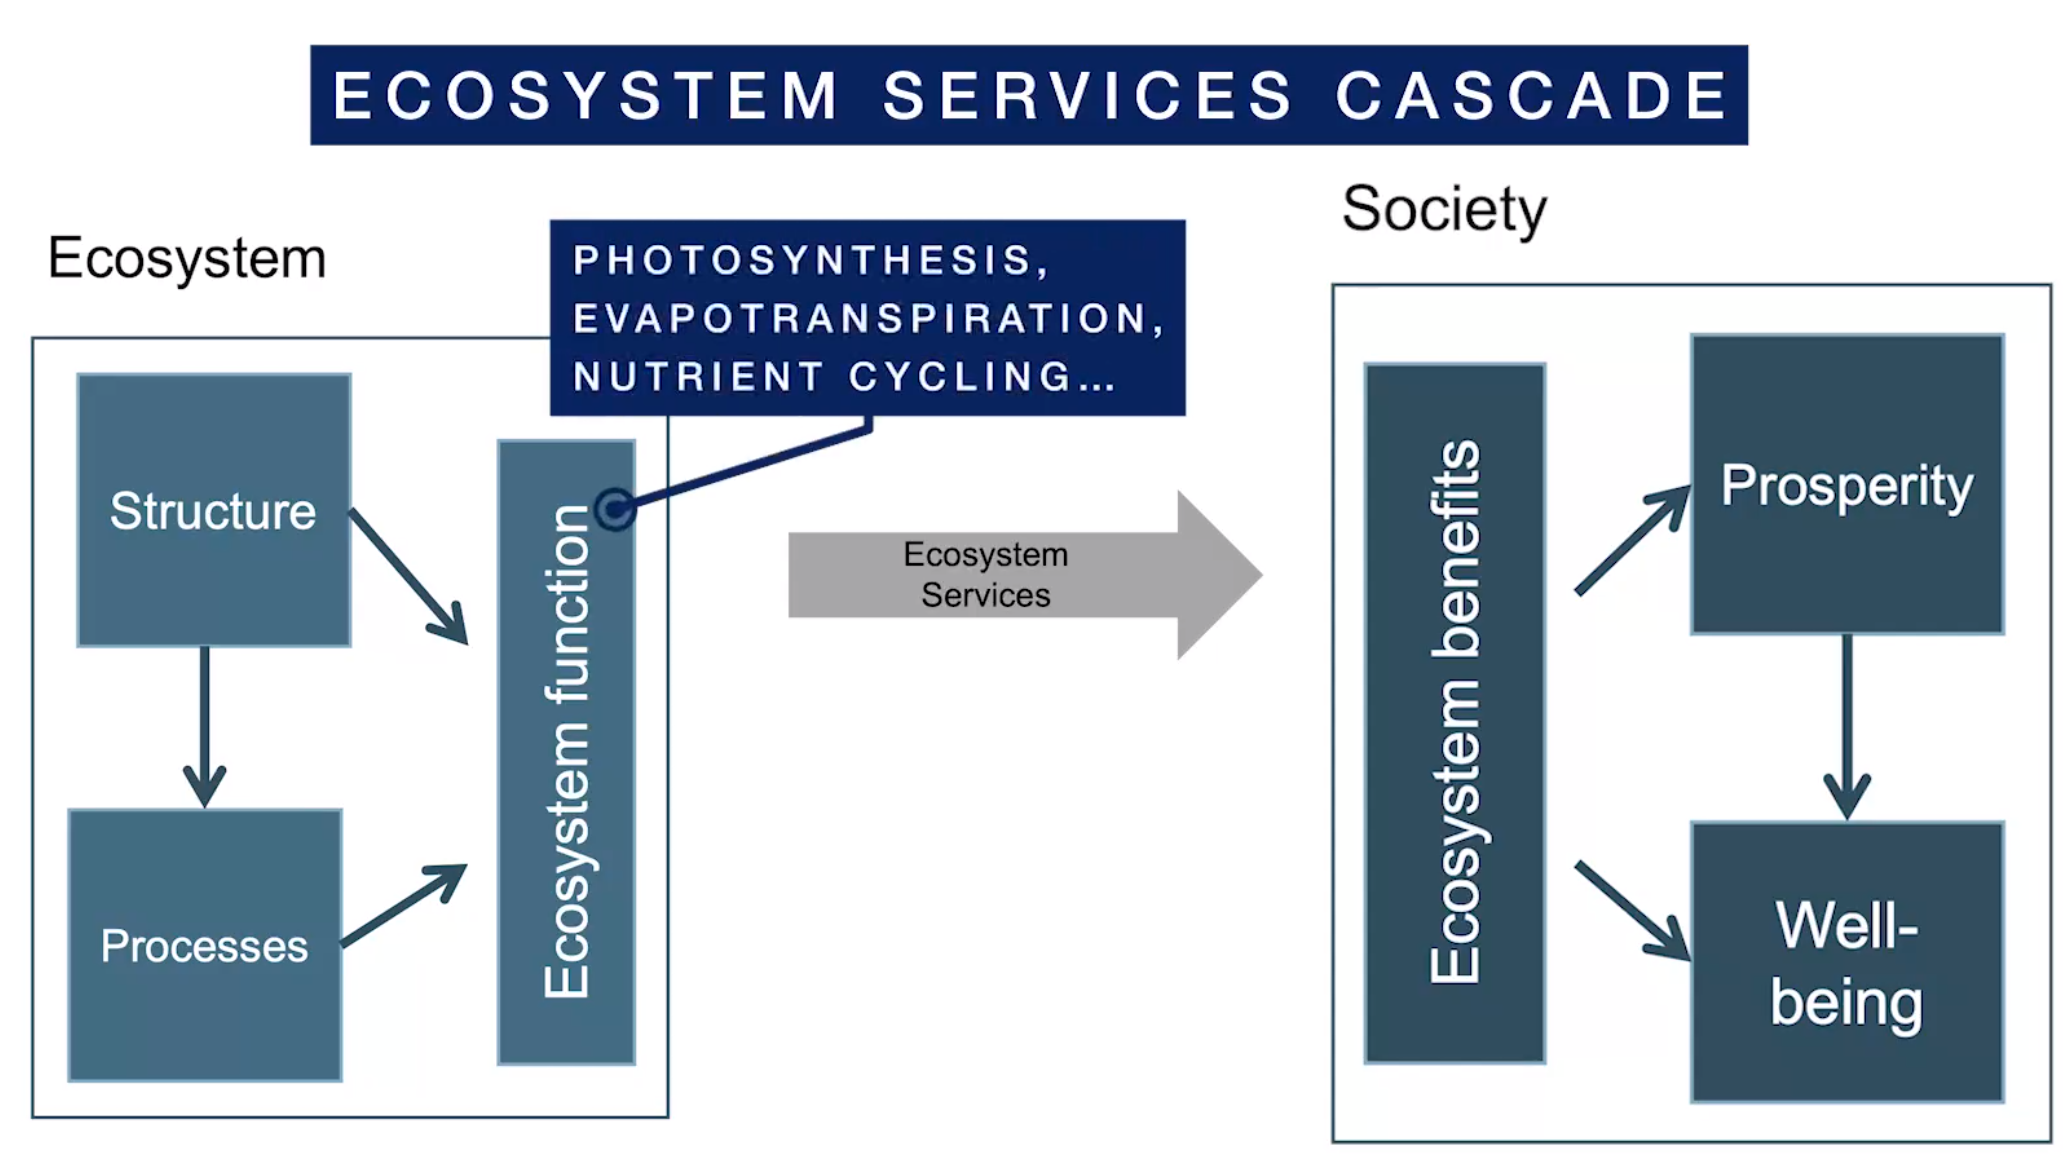
\includegraphics[width=0.9\linewidth]{images/2-ecosystem-services-cascade.png}
		\caption{Ecosystem Services cascade}
		\label{fig:ecosystems_services_cascade}
	\end{figure}
	
	\newpage
	\ \\
	There is a \textbf{positive but asymptotic} biodiversity – ecosystem service relationship. This relationship is visualised in Figure \ref{fig:relationship_biodiversity_ecosystems_services}. This means that increasing biodiversity leads to an increase in ecosystem service performance up to a certain extent, after which adding more biodiversity does not much further increase the service provision. It also means that losing some biodiversity as a consequence of human ecosystem degradation may not directly lead to large losses in ecosystem services, but that a further degradation over a critical threshold of species loss will lead to strong reductions in ecosystem services.
	
	\begin{figure}[htbp]
		\centering
		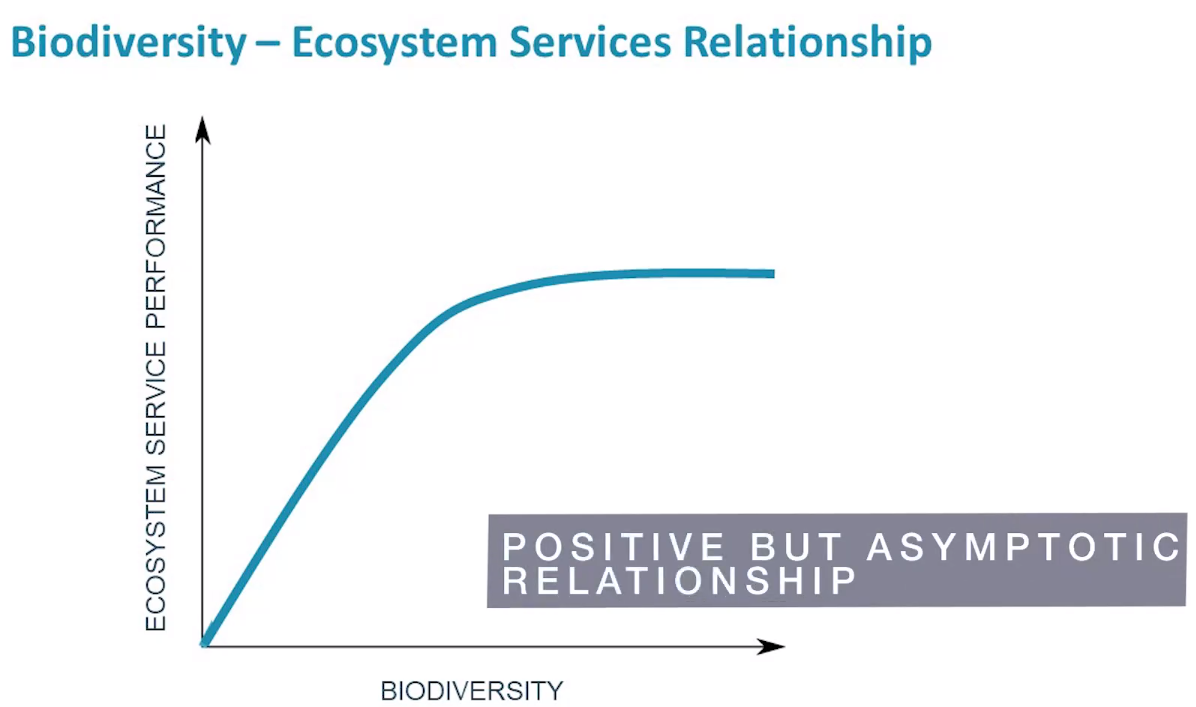
\includegraphics[width=0.9\linewidth]{images/2-biodiversity-ecosystem-services-relationship.png}
		\caption{Relationship between biodiversity and ecosystems services}
		\label{fig:relationship_biodiversity_ecosystems_services}
	\end{figure} 	
	\ \\
	Nowadays, IPBES, the Intergovernmental Science-Policy Platform on Biodiversity and Ecosystem Services, speaks about \textbf{Nature's Contributions to People (NCP)}, which are all the contributions, both positive and negative, of living nature, which includes the diversity of organisms, ecosystems, and their associated ecological and evolutionary processes, to the quality of life for people.
	
	\newpage
	
	\subsection{How to measure biodiversity and what are the challenges}
	\subsubsection{Challenges}
	To directly measure the effect of a human intervention on the level of biodiversity, we require evidence of a clear \textbf{causal relationship} between intervention and impact (change in biodiversity is caused by the human intervention), the \textbf{absence of other confounding factors} (human intervention the only thing that is influencing) and clear decisions on \textbf{which elements of biodiversity} are considered. 
	\\
	\\
	Hence, measuring and monitoring biodiversity is very complex. For this reason often simplified proxies for biodiversity are used, e.g. \textbf{indicator species}, which are known to be sensitive for certain human-induced disturbances, or \textbf{multi-taxa approaches}, to sense the impact on different groups of organisms. Measuring the different dimensions of biodiversity requires a combination of different techniques from regional coverage using satellites to local ground coverage using camera traps or citizen science. 
	\\
	\\
	In order to create some structure in this multitude of information, the international community (GEO-BON) developed a framework of Essential Biodiversity Variables (EBV) including the following classes: \textbf{genetic composition, species populations,  species traits, community composition, ecosystem structure and ecosystem functioning}.
	
	\subsubsection{Measure biodiversity}
	Monitoring species population is today the most common indicator method. Observations from experts and citizen science are brought together in the GBIF global biodiversity database. This data together with other data sources are used to build and update \textbf{IUCN Red List}, visualized in figure \ref{fig:iucn-red-list}, as the major indicator tool for global biodiversity loss.
	\\
	\\
	This indicator tool monitors the extinction risk of individual species. Based on objective criteria, species are assigned to one of the 6 classes in the red list going from least concern for species with the lowest risk of extinction to species that are globally extinct. The individual species status information can then be brought together synthesis indices, like WWFs \textbf{Living Planet Index} (LPI). As explained in figure \ref{fig:living-planet-index}.
	
	\begin{figure}[H]
		\centering
		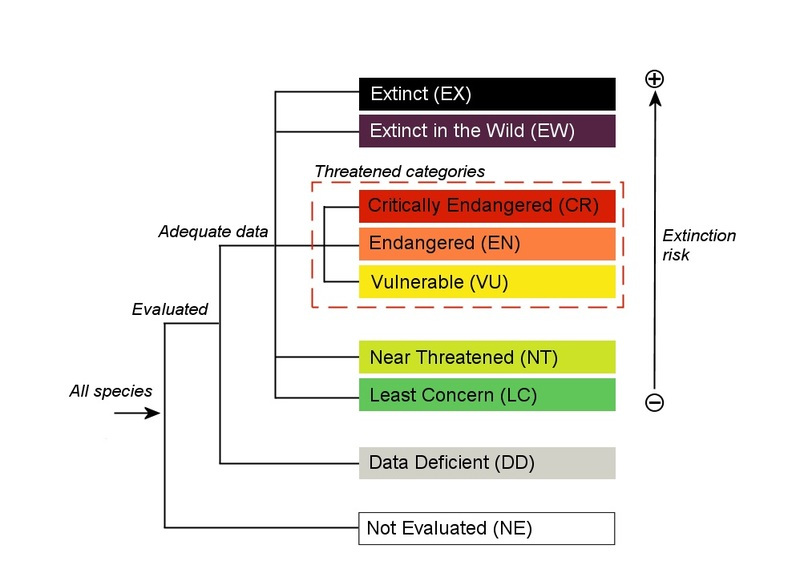
\includegraphics[width=0.6\linewidth]{../images/2-IUCN-red-list}
		\caption{The IUCN Red List - indicates how close a species is to becoming extinct}
		\label{fig:iucn-red-list}
	\end{figure}
	
	\newpage
	\ \\
	A very different approach is to measure so-called \textbf{mid-point indicators}. They do not measure the biodiversity loss itself, but rather quantify the frequency and intensity of the damaging interventions. These indicators assume a known relationship between intervention and effect, which is a rather rough approach. Their advantage is that they are much cheaper and have much better data availability than measuring biodiversity effects itself. Examples are area impacted by irrigation, fertilization, biocide use,… .
	\\
	\\
	This approach is typical for \textbf{Land Use Impact methods} used in \textbf{LCA (Life Cycle Assessment)} and \textbf{Environmental Footprint Analysis} , which calculate the impact of land use change (e.g. deforestation) or of permanent land use (e.g. long-term cropland) by measuring the loss of land quality over time for a certain area, see figure \ref{fig:mid-point-indicator}.
	(Land use change $\rightarrow$ Strong decline in small period \& Permanent land use $\rightarrow$ less strong decline for a long
	period)	
	\begin{figure}[H]
		\centering
		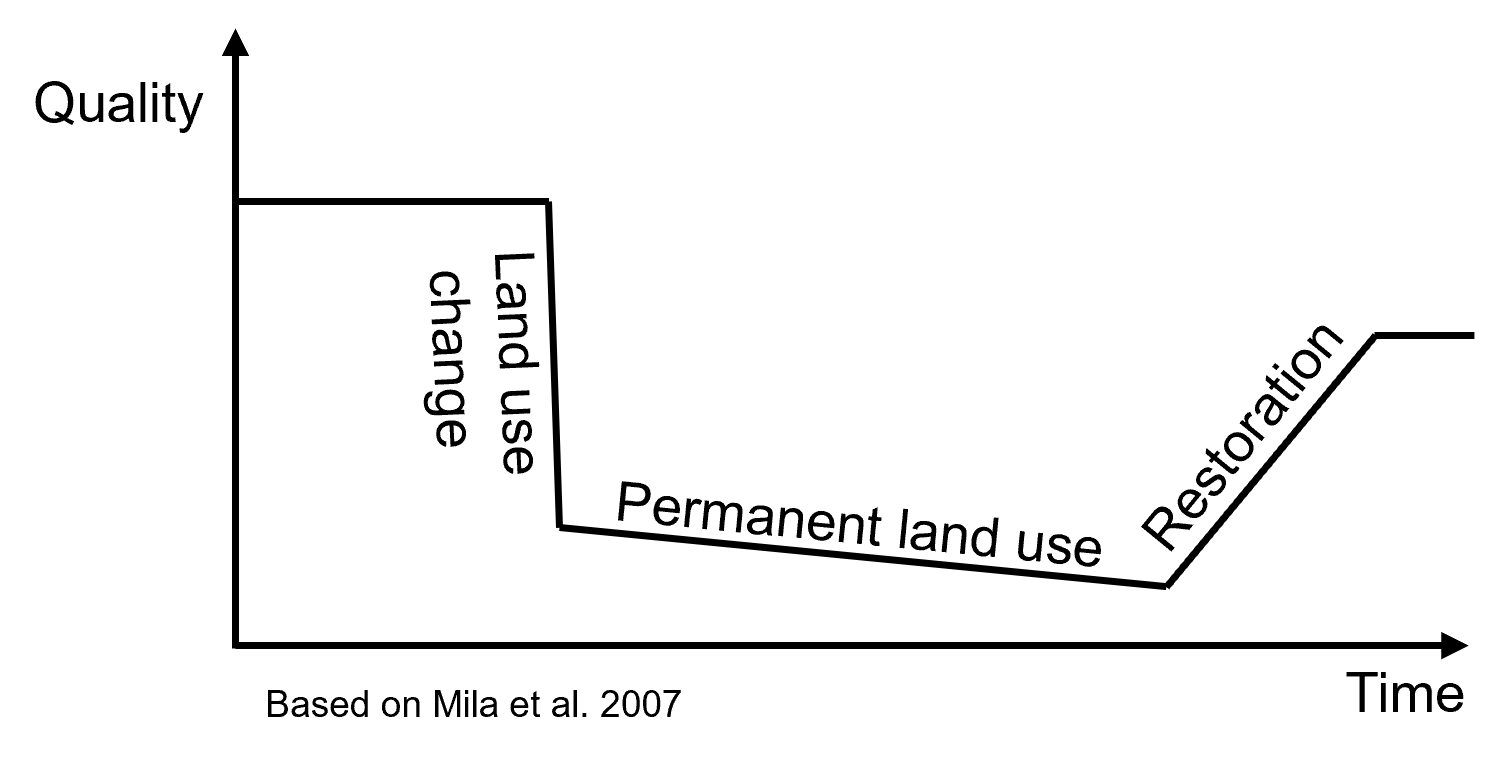
\includegraphics[width=0.6\linewidth]{../images/2-mid-point-indicator}
		\caption{Evolution of land quality with land use interventions}
		\label{fig:mid-point-indicator}
	\end{figure}
	
	
	\subsection{Treats for biodiversity} 
	The main threats to biodiversity can be categorized in 5 different drivers, referred to as the \textbf{evil quintet}. In decreasing order of importance these are habitat loss, overexploitation through hunting and fishing, climate change, pollution and invasive species. Apart from these threats there are other threats that do not fit clearly into these categories, such as for example wildfire or direct human disturbances due to recreational activities.
	\\
	\\
	\textbf{Habitat loss} refers to the transformation of natural habitats into other land uses. It is mainly caused by expanding agricultural land which is especially problematic in the tropics and subtropics.
	\\
	\\
	\textbf{Overexploitation} through hunting and fishing is the second most important threat. It can happen for food or for valued body parts such as ivory.
	\\
	\\
	\textbf{Climate change} is a newly emerging threat to biodiversity. The climate can become too hot or too dry for a species to persist. And very often northward migration of the species to a more mild climate is hampered through habitat loss.
	\\
	\\
	\textbf{Pollution} mainly refers to the effects of agrochemicals such as pesticides and the effects of overuse of fertilizers.
	\\
	\\
	\textbf{Invasive} (or exotic or non-native) \textbf{species} may outcompete or predate the indigenous species. They can also introduce new diseases and pests. This as opposed to \textbf{indigenous} (or native) \textbf{species}. \\
	\textbf{Invasive alien species} (IAS) are non-native species that cause economic or environmental harm or adversely affect human health.  \\
	Alien species can be introduced in many ways. Usually we divide them into \textbf{unintentional/accidental and intentional introductions}. 

	\subsection{Restoring biodiversity}
	There are a couple ways we can try to conserve and restore biodiversity. It is based on the idea that there are two main ways to reduce the impacts of farming on wild species. The first is making the farmland itself more wildlife-friendly (this is land sharing), the second is making more space for natural or unfarmed habitats (this is land sparing).
	\\
	\\
	\textbf{Land sharing} or nature friendly farming (left on Figure \ref{fig:land-sharing-sparing}) involves integrating practices which benefit biodiversity (such as retaining important habitat features like ponds and hedges) within the area producing the food. There is however a limit to how friendly one can make farmland for wild species without reducing the yields too much, and lower yields mean that more land is needed to produce each ton of food, making it harder to create more space for nature.
	\\
	\\
	\textbf{Land sparing} on the other hand (right on Figure \ref{fig:land-sharing-sparing}) starts from the observation that high-yielding agriculture can reduce the area needed to meet a given level of demand for food. Land sparing will concentrate higher-yielding production in some parts of the landscape while simultaneously retaining or restoring other parts of the landscape for nature.
	\\
	\\
	When studying this model, the key finding is \textbf{that most species would have larger populations if a given amount of food is produced on as small an area as possible, while sparing as large an area of native vegetation as possible}. 
	\\
	\begin{figure}[htbp]
		\centering
		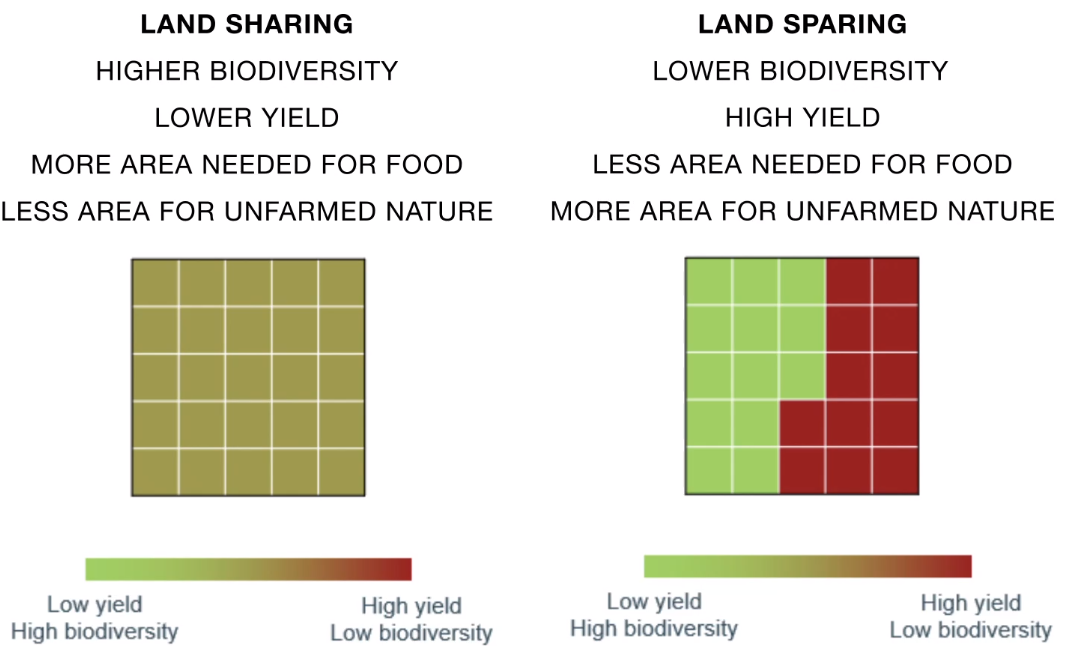
\includegraphics[width=0.8\linewidth]{images/2-land-sharing-sparing.png}
		\caption{Land sharing versus land sparing}
		\label{fig:land-sharing-sparing}
	\end{figure}
	\ \\
	A second subject we can study, is human activity. \textbf{Ecological restoration} is the process of \textbf{assisting the recovery of damaged, degraded, or destroyed ecosystems}. Restoration aims to reverse damage and protect the biodiversity and services that ecosystems provide.
	\\
	\\
	Recently, \textbf{rewilding} has emerged as a new approach to ecosystem restoration. It promotes "wild, autonomous" nature, with natural processes driven by keystone species and abiotic processes leading the way instead of human intervention. Some examples of common approaches employed in rewilding initiatives are the \textbf{reintroduction of large fauna species or trophic rewilding, restoring habitat connectivity, wetland restoration and natural regeneration and succession}. 
	
\end{document}
